% !TeX TXS-program:compile = txs:///pdflatex/[--shell-escape]
\documentclass[]{article}
\usepackage{polski}
\usepackage[utf8]{inputenc}
\usepackage{graphicx}
\usepackage{wrapfig}
\usepackage{float}
\graphicspath{{./zdjecia/}}


% Title Page
\title{Sprawozdanie Lab 3}
\author{Wojciech Kosierkiewicz 272926}
%python config
% !TeX TXS-program:compile = txs:///pdflatex/[--shell-escape]
\usepackage{tcolorbox}
\tcbuselibrary{minted,breakable,xparse,skins}

\definecolor{bg}{gray}{0.95}
\DeclareTCBListing{mintedbox}{O{}m!O{}}{%
  breakable=true,
  listing engine=minted,
  listing only,
  minted language=#2,
  minted style=default,
  minted options={%
    linenos,
    gobble=0,
    breaklines=true,
    breakafter=,,
    fontsize=\small,
    numbersep=8pt,
    #1},
  boxsep=0pt,
  left skip=0pt,
  right skip=0pt,
  left=25pt,
  right=0pt,
  top=3pt,
  bottom=3pt,
  arc=5pt,
  leftrule=0pt,
  rightrule=0pt,
  bottomrule=2pt,
  toprule=2pt,
  colback=bg,
  colframe=orange!70,
  enhanced,
  overlay={%
    \begin{tcbclipinterior}
    \fill[orange!20!white] (frame.south west) rectangle ([xshift=20pt]frame.north west);
    \end{tcbclipinterior}},
  #3}

% !TeX TXS-program:compile = txs:///pdflatex/[--shell-escape]


\begin{document}
	\maketitle
	\newpage
	
\section{Wstęp}
Podczas tych laboratoriów uczyłem się jak tworzyć obiekty 3D. Zadania które musiałem wykonać polegały na stworzeniu jajka w 3 wymiarach i wyświetlenie go na różne sposoby. Pierwsze przez kropki, potem przez linie a następnie przez trójkąty. W ostatnim zdaniu musiałem użyć Triangle strip. Jajko musiało być nieprzerwane oraz obracać się podczas wyświetlania.
\section{Zadania}
\subsection{zadanie 1}
By wykonać zadanie pierwsze musiałem pierwsze stworzyć macierz w której będę mógł przechowywać wszystkie swoje punkty a następnie uzupełnić ją punktami w odpowiednich pozycjach na osiach x,y i z. Na szczęście nie jestem pierwszą osobą która chciała malować jajka i matematycy stworzyli wzory podwalające na wyliczenie koordynatów każdego z punktów. Te wzory zostały zaimplementowane poniżej.
\begin{figure}[H]
	\begin{minted}{python}
def getx(u,v):
    return (-90 * pow(u,5)+225 * pow(u,4) -270 * pow(u,3)
     + 180 * u*u - 45*u)*math.cos(math.pi*v)

def gety(u,v):
    return (160 * pow(u,4) - 320 * pow(u,3)
     + 160 * u * u - 5)

def getz(u,v):
    return (-90 * pow(u,5) + 225 * pow(u,4) - 270 * pow(u,3)
     +180 * pow(u,2) - 45*u) * math.sin(math.pi*v)
\end{minted}
\caption{Funkcje użyte do generowania punktów}
\end{figure}
Powyżej napisane funkcje wywoływałem dla każdego punktu jajka którego chciałem wyświetlić i przypisałem do macierzy.
\begin{figure}[H]
	\begin{minted}{python}
N = 100
points = [[[0] * 3 for i in range(N)] for j in range(N)];

def fillpoints(N):
    for i in range(N):
        for j in range(N):
            if i != 0 and j != 0:
                points[i][j][0]= getx(i/N,j/N)
                points[i][j][1]= gety(i/N,j/N)
                points[i][j][2]= getz(i/N,j/N)
	\end{minted}
\end{figure}
Posiadając już wszystkie punkty tworzące moje jajko pozostało mi jedynie je wyświetlić oraz obracać. Zrobiłem oba w poniższym kodzie. Funkcja spin odpowiadała za obrót jajka w wszystkich osiach o podany kąt w zmiennej angle. Podczas wyświetlania używałem czasu do obliczania kątu obrotu.
\begin{figure}[H]
\begin{minted}{python}
def spin(angle):
    glRotatef(angle,1.0,0.0,0.0)
    glRotatef(angle,0.0,1.0,0.0)
    glRotatef(angle,0.0,0.0,1.0)

def render(time):
    glClear(GL_COLOR_BUFFER_BIT | GL_DEPTH_BUFFER_BIT)
    glLoadIdentity()
    spin(time * 180 / 3.1415)
    glPointSize(5)
    axes()
    glBegin(GL_POINTS)
    for i in range(N):
        for j in range(N):
            glColor3f(random.uniform(0,1),random.uniform(0,1),random.uniform(0,1))
            glVertex3f(points[i][j][0],points[i][j][1],points[i][j][2])
    glEnd()
    glFlush()
	
\end{minted}
\end{figure}
Efektem końcowym było jajko stworzone z pojedynczych kolorowych punktów. 
\begin{figure}[H]

	\centering
	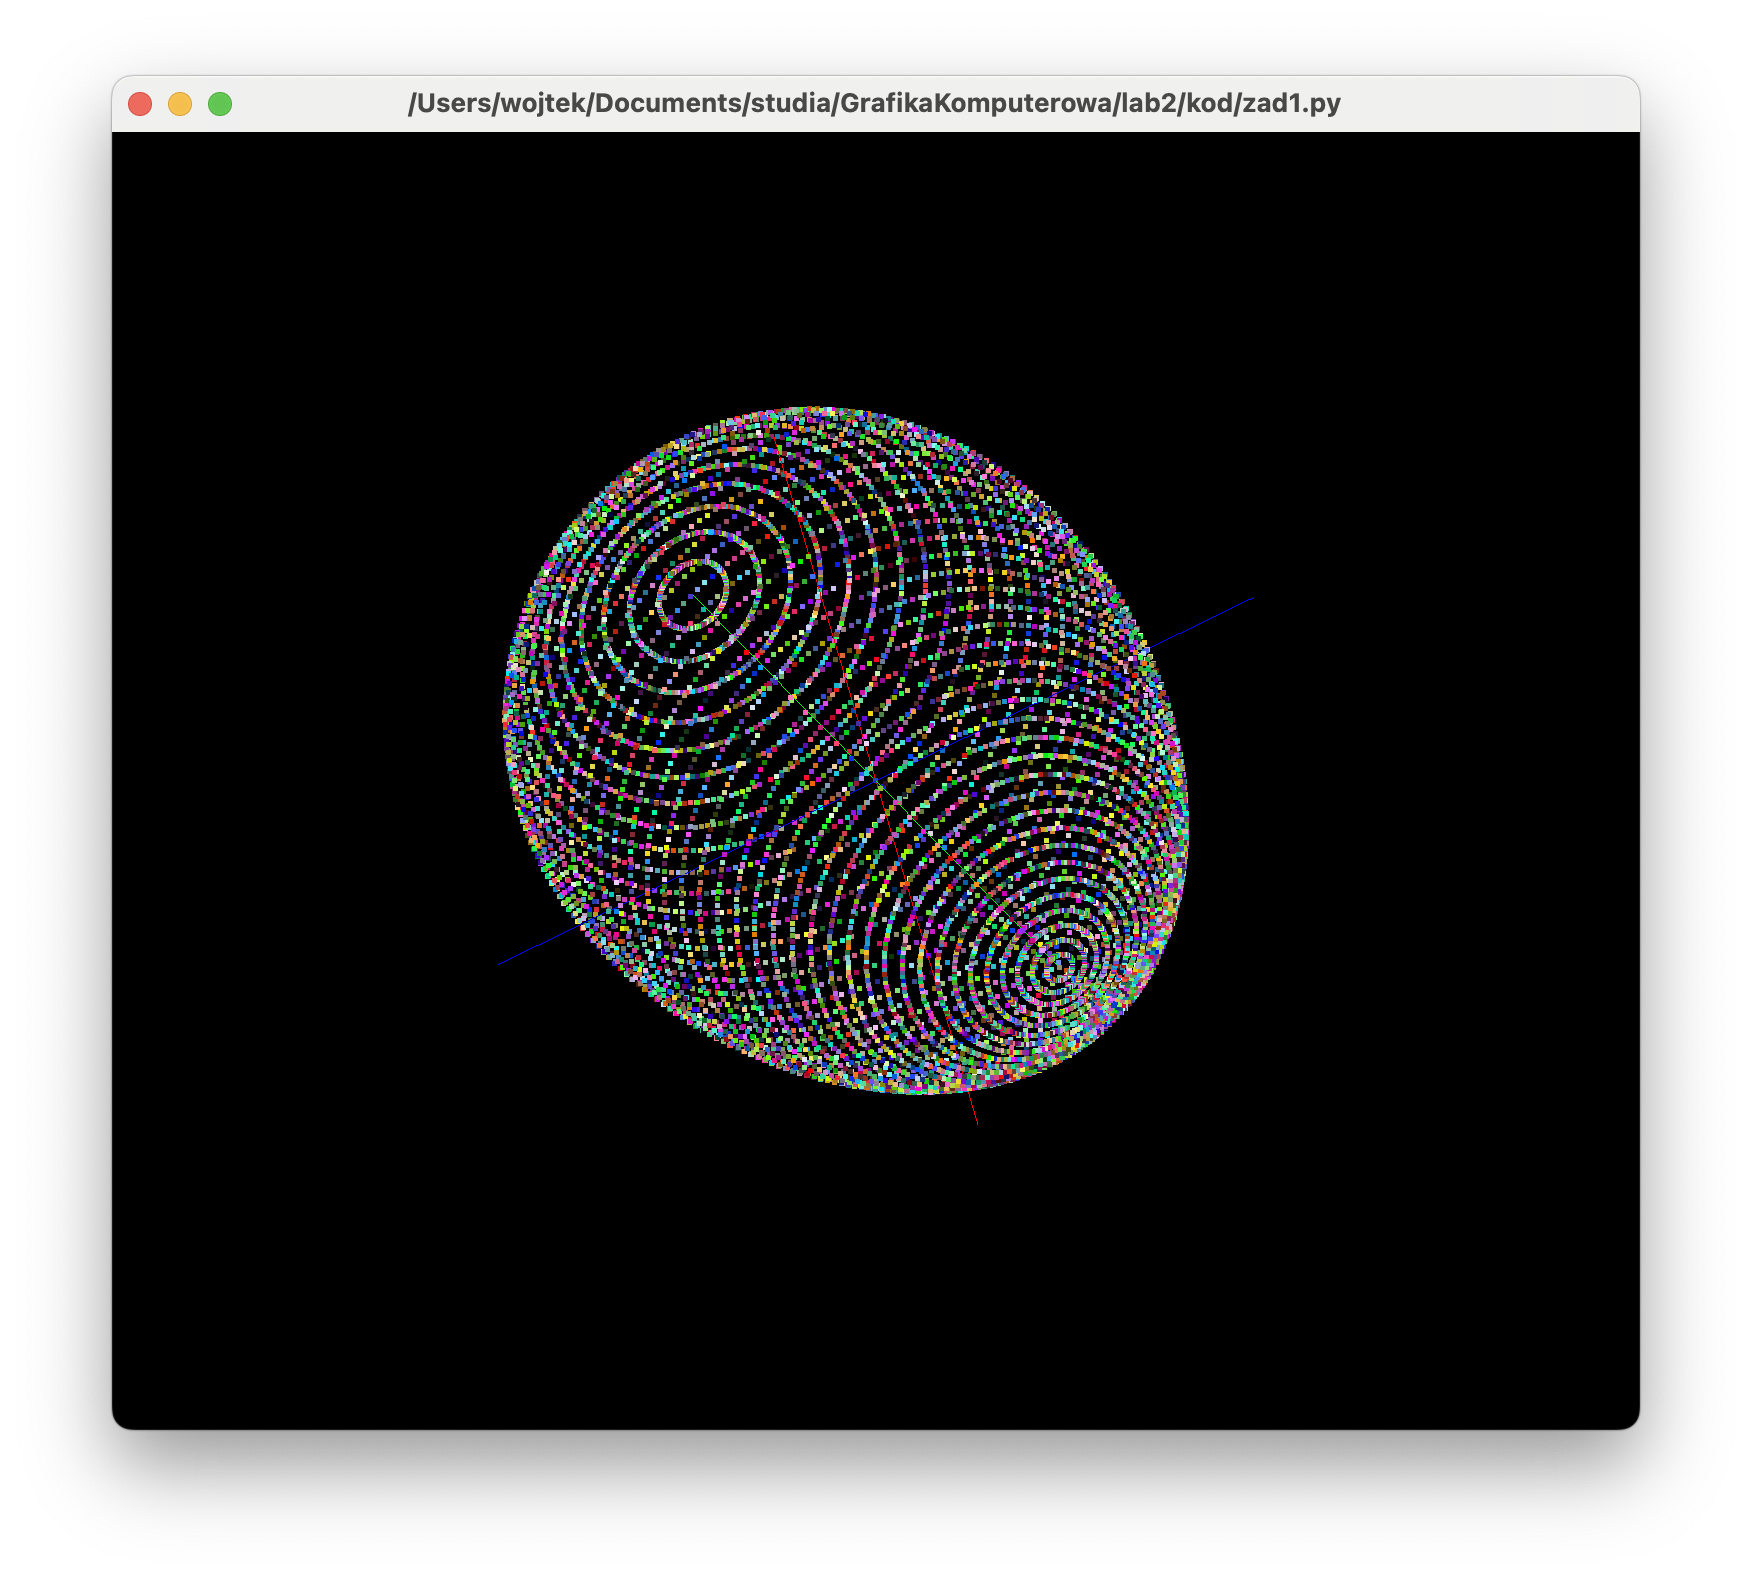
\includegraphics[width=\textwidth]{zad1.png}
	\caption{Wynik zadania 1}
\end{figure}
\subsection{zadanie 2}
W zadaniu 2 mogłem ponownie wykorzystać większość mojego poprzedniego kodu ale musiałem zmienić kolejność wyświetlania elementów by móc uzyskać połączone jajko. Dlatego dodawałem po dwa połączenia dla każdego punktu. Pierwsze połączenie $(i,j)\rightarrow (i+1,j)$ a potem $(i,j) \rightarrow (i,j+1)$.
\begin{figure}[H]
	\begin{minted}{python}
glBegin(GL_LINES)
for i in range(N)
	for j in range(N):
		#(i,j)->(i+1,j)
		glVertex3f(points[i][j][0],points[i][j][1],points[i][j][2])
		glVertex3f(points[i+1][j][0],points[i+1][j][1],points[i+1][j][2])
		#(i,j)->(i,j+1)
		glVertex3f(points[i][j][0],points[i][j][1],points[i][j][2])
		glVertex3f(points[i][j+1][0],points[i][j+1][1],points[i][j+1][2])
	\end{minted}
\end{figure}
Dzięki takiej kolejności dodawaniu punktów do wyświetlania uzyskałem jajko stworzona z połączonych lini. By uzyskać losowe kolory bez migotania stworzyłem drugą identyczną macierz do tej w której przechowywałem pozycje punktów i wypełniałem ją losowymi kolorami które potem używałem do kolorowania każdej z linii.
\begin{figure}[H]
	\begin{minted}{python}
clrs = [[[0.0] * 3 for i in range(N+1)] for j in range(N+1)];
def colors(N):
    for i in range(N+1):
        for j in range(N+1):
            random.seed(i*j)
            clrs[i][j][0]= random.uniform(0.0,1.0)
            clrs[i][j][1]= random.uniform(0.0,1.0)
            clrs[i][j][2]= random.uniform(0.0,1.0)
	\end{minted}
\end{figure}
\begin{figure}[H]
	\centering
	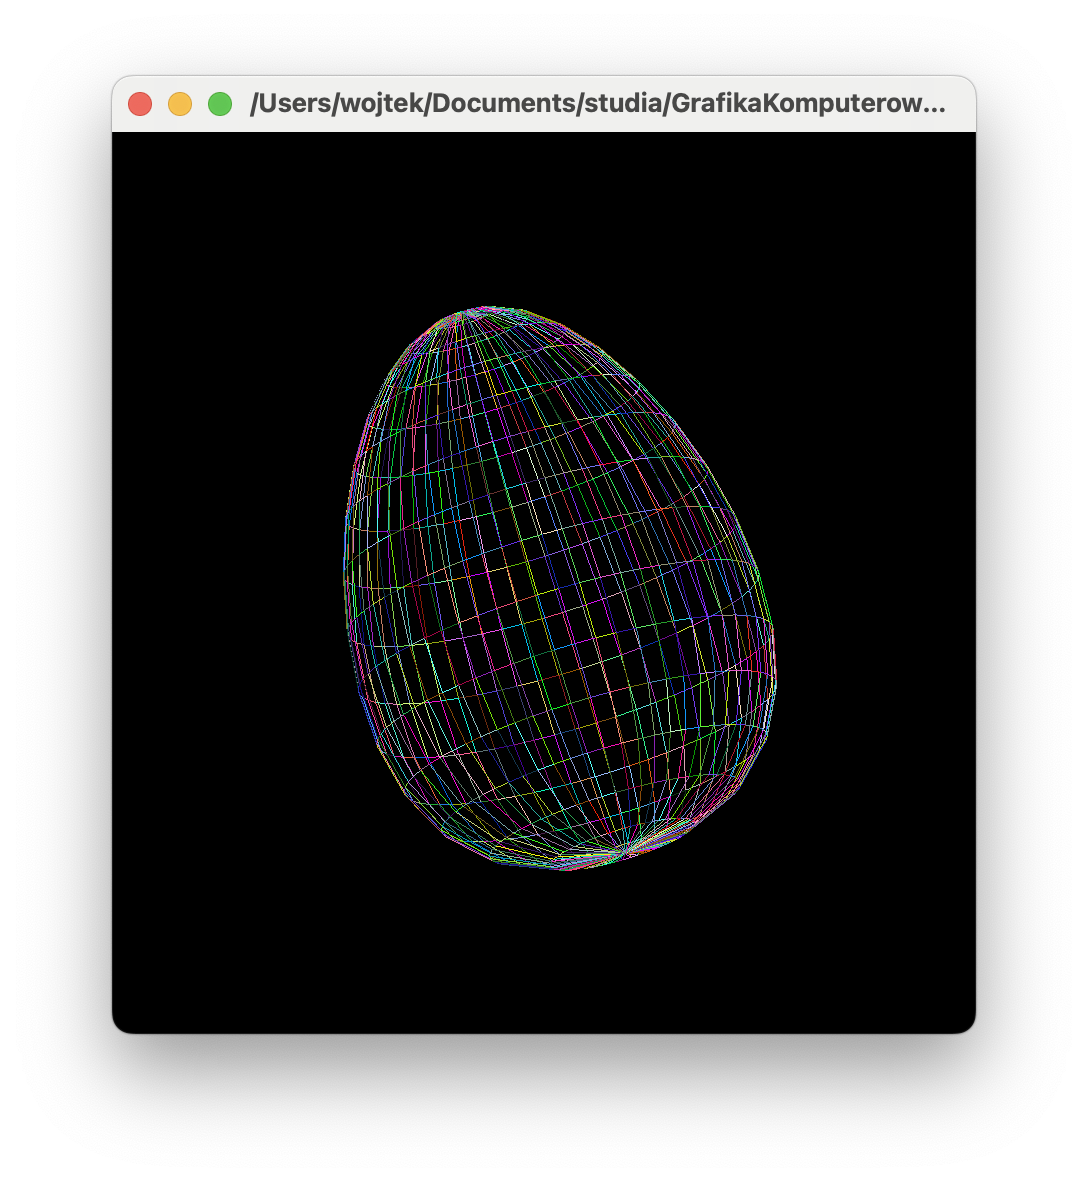
\includegraphics[width=\textwidth]{zad2.png}
	\caption{Wynik zadania 2}
\end{figure}
\subsection{zadanie 3}
Jedyne konieczne zmiany w zadaniu 3 były w kolejności wyświetlania. Natomiast dowiedziałem się także o możliwości użycia funkcji glVertex3fv zamiast glVertex3f która przyjmuje całą macierz współrzędnych na raz zamiast przekazywania każdego elementu. Natomiast by wyświetlić wszystkie prostokąty używając trójkątów musiałem stworzyć dwa trójkąty dzielące ze sobą wierzchołki $(i,j+1),(i+1,j)$ ale 3 wierzchołek musiał być przeciwny, tworzyłem więc dwa trójkąty o współrzednych $(i,j),(i+1,j),(i,j+1)$ , $(i+1,j+1),(i+1,j),(i,j+1)$.
\begin{figure}[H]
	\begin{minted}{python}
glBegin(GL_TRIANGLES)
for i in range(N):
	for j in range(N):
		glColor3fv(clrs[i+1][j+1])
		#pierwszy trójkąt
		glVertex3fv(points[i][j])
		glVertex3fv(points[i+1][j])
		glVertex3fv(points[i][j+1])
		#drugi trójkąt
		glVertex3fv(points[i+1][j+1])
		glVertex3fv(points[i][j+1])
		glVertex3fv(points[i+1][j])
	\end{minted}
\end{figure}
\begin{figure}[H]
	\centering
	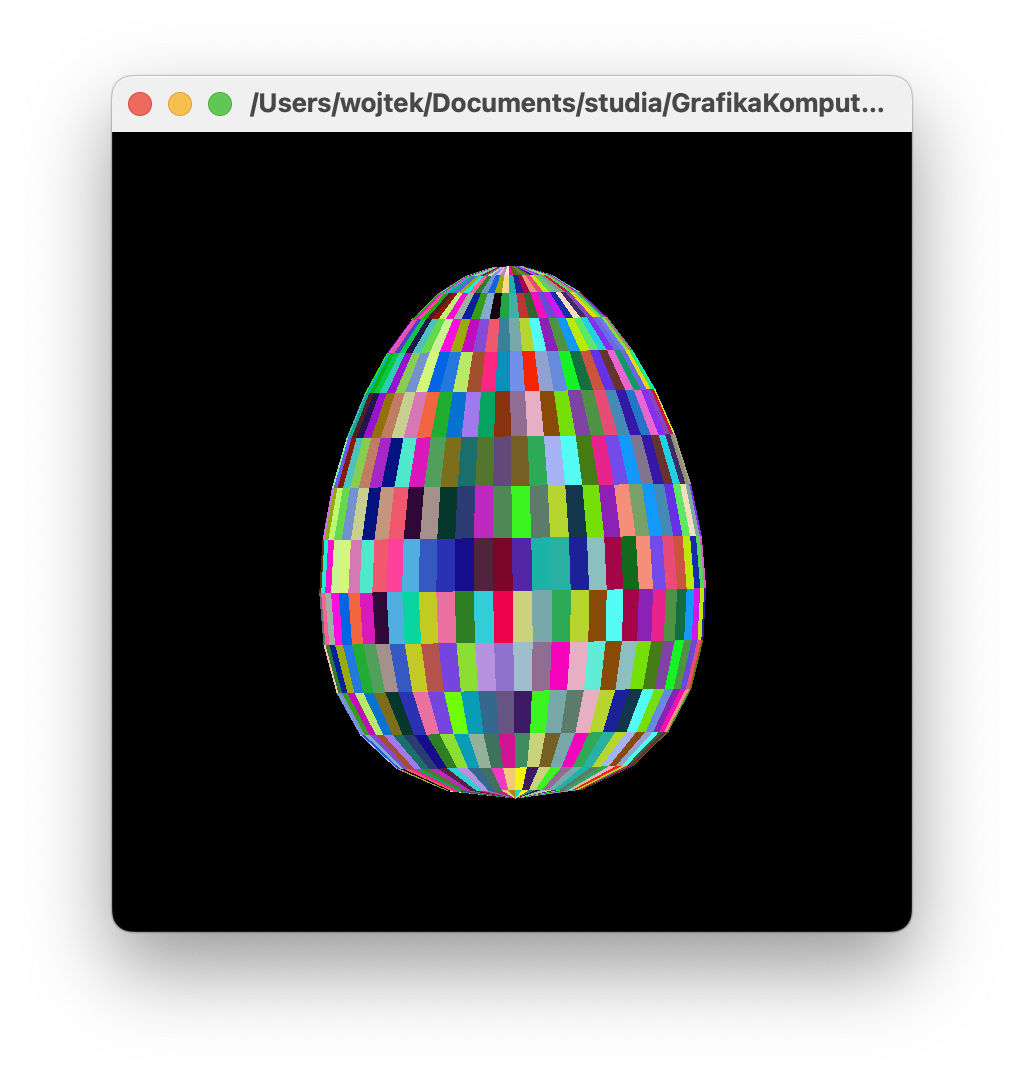
\includegraphics[width=\textwidth]{zad3.png}
	\caption{Wynik zadania 3}
\end{figure}
\subsection{zadanie 4}
Zadanie 4 nie było trudne i jedynie wymagało przekazywania na przemian punktów z górnego i dolnego wiersza. wykonałem to w poniższym kodzie.
\begin{figure}
	\begin{minted}{python}
for i in range(N):
	for j in range(N):
		glColor3fv(clrs[i+1][j+1])
		
		glVertex3fv(points[i][j])
		glVertex3fv(points[i+1][j])
		glVertex3fv(points[i][j+1])
		glVertex3fv(points[i+1][j+1])
	\end{minted}
\end{figure}
\begin{figure}[H]
	\centering
	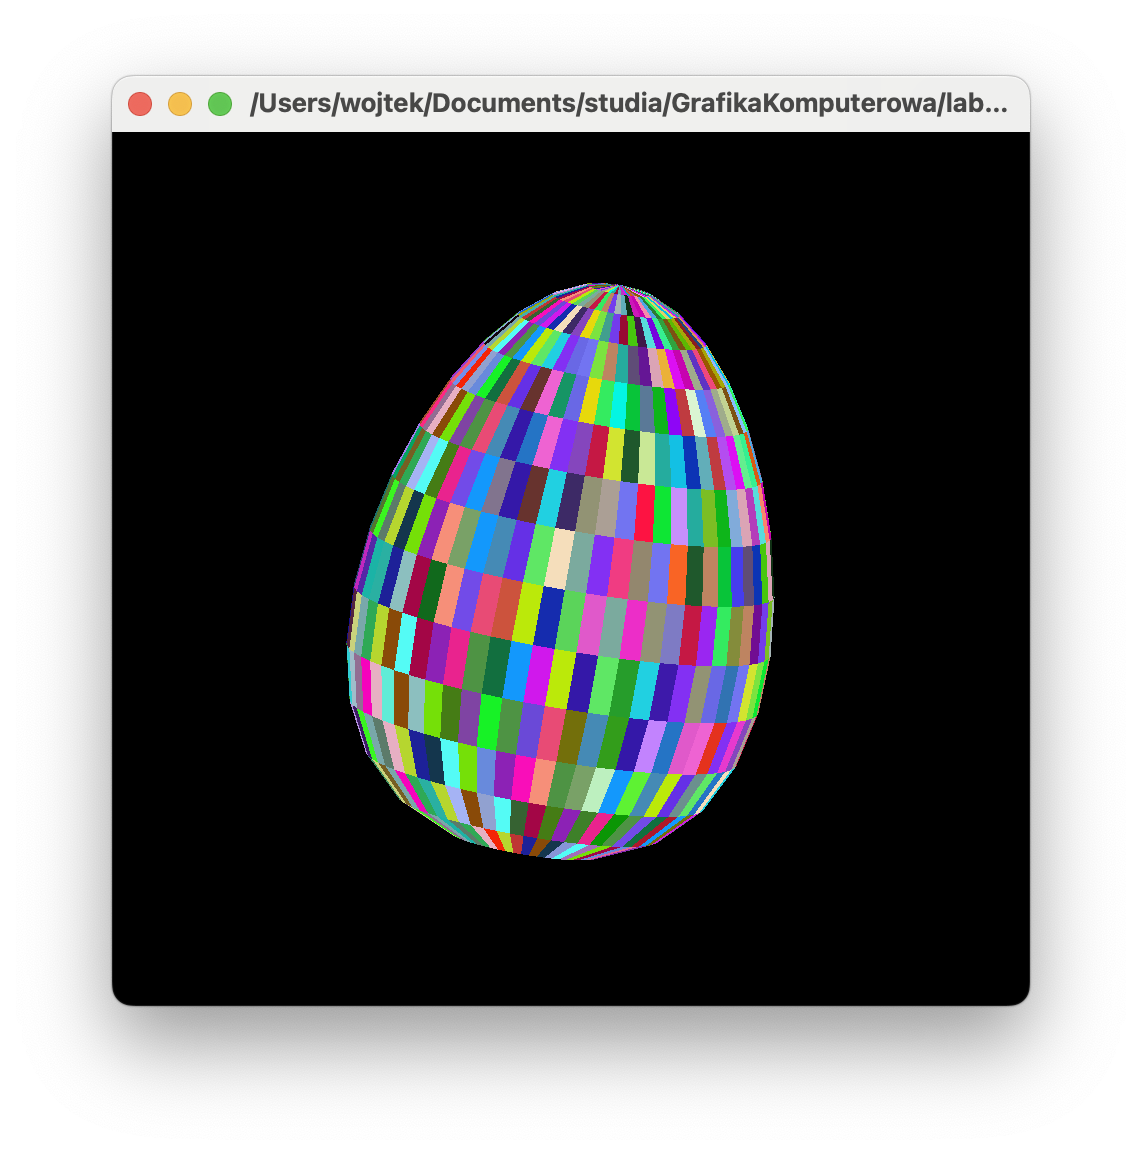
\includegraphics[width=\textwidth]{zad4.png}
	\caption{Wynik zadania 4}
\end{figure}
\section{wnioski}
Obsługa obiektów 3D nie jest dużo trudniejsza od obsługi obiektów 2D. Wszystkie funkcje są zaskakująco podobne. 
\end{document}          
